\documentclass[10,letterpaper,]{report}
\usepackage[T1]{fontenc}
\usepackage{lmodern}
\usepackage{float}
\usepackage{titlesec}
\usepackage{amssymb,amsmath}
\usepackage{ifxetex,ifluatex}
\usepackage[export]{adjustbox}
\usepackage{tikz} 
\usepackage{fixltx2e} % provides \textsubscript



% use upquote if available, for straight quotes in verbatim environments
\IfFileExists{upquote.sty}{\usepackage{upquote}}{}
\ifnum 0\ifxetex 1\fi\ifluatex 1\fi=0 % if pdftex
  \usepackage[utf8]{inputenc}
\else % if luatex or xelatex
  \usepackage{fontspec}
  \ifxetex
    \usepackage{xltxtra,xunicode}
  \fi
  \defaultfontfeatures{Mapping=tex-text,Scale=MatchLowercase}
  \newcommand{\euro}{€}
  \setmainfont{Adobe Caslon Pro}
  \setsansfont{Myriad Pro Bold Condensed}
\fi
% use microtype if available
\IfFileExists{microtype.sty}{\usepackage{microtype}}{}




% COLIN CHANGES



\usepackage[margin=1in]{geometry}


% See p.105 of "TeX Unbound" for suggested values.
% See pp. 199-200 of Lamport's "LaTeX" book for details.
%   General parameters, for ALL pages:
\renewcommand{\topfraction}{0.9}  % max fraction of floats at top
\renewcommand{\bottomfraction}{0.8} % max fraction of floats at bottom
%   Parameters for TEXT pages (not float pages):
\setcounter{topnumber}{2}
\setcounter{bottomnumber}{2}
\setcounter{totalnumber}{4}     % 2 may work better
\setcounter{dbltopnumber}{2}    % for 2-column pages
\renewcommand{\dbltopfraction}{0.9} % fit big float above 2-col. text
\renewcommand{\textfraction}{0.07}  % allow minimal text w. figs
%   Parameters for FLOAT pages (not text pages):
\renewcommand{\floatpagefraction}{0.7}  % require fuller float pages
% N.B.: floatpagefraction MUST be less than topfraction !!
\renewcommand{\dblfloatpagefraction}{0.7} % require fuller float pages

\usepackage{caption}
\captionsetup[figure]{name={Figure.}}
\captionsetup{font={rm,small,singlespacing,bf},justification=RaggedRight}

\usepackage{setspace}
\setstretch{1.2}

\newfontfamily{\myriadpcondensed}{Myriad Pro Condensed}
\newfontfamily{\myriadpcondensedbold}{Myriad Pro Bold Condensed}

\usepackage{sectsty}
%\sectionfont{\normalfont\myriadpcondensedbold\fontsize{50}{60}\selectfont}
\sectionfont{\normalfont\myriadpcondensedbold\huge}
\subsectionfont{\normalfont\myriadpcondensed\LARGE}

%\usepackage[top=20mm, bottom=70mm, left=18mm, right=18mm]{geometry}


\usepackage[english]{babel}
%\usepackage{fancyhdr}

%\fancyhf{}
%\fancyhead[L]{}

%\renewcommand{\headrulewidth}{0pt}
%\renewcommand{\footrulewidth}{0pt}
%\setlength\headheight{30pt}

%\pagestyle{fancy}

\titlespacing\section{0pt}{12pt plus 4pt minus 2pt}{0pt plus 2pt minus 2pt}
\titlespacing\subsection{0pt}{12pt plus 4pt minus 2pt}{0pt plus 2pt minus 2pt}
\titlespacing\subsubsection{0pt}{12pt plus 4pt minus 2pt}{0pt plus 2pt minus 2pt}

\titleformat{\chapter}[display]
{\sffamily\Huge\bfseries}{}{-70pt}{\fontsize{45}{100}\selectfont}

% this alters "before" spacing (the second length argument) to 0
\titlespacing*{\chapter}{0pt}{0pt}{40pt}


\usepackage{xcolor} % Required for specifying custom colors
\usepackage{fix-cm} % Allows increasing the font size of specific fonts beyond LaTeX default specifications

\setlength{\oddsidemargin}{0mm} % Adjust margins to center the colored title box
\setlength{\evensidemargin}{0mm} % Margins on even pages - only necessary if adding more content to this template

\newcommand{\HRule}[1]{\hfill \rule{0.2\linewidth}{#1}} % Horizontal rule at the bottom of the page, adjust width here



%\makeatletter
%\def\@makechapterhead#1{%
%  \vspace*{50\p@}%
%  {\parindent \z@ \raggedright
%    \interlinepenalty\@M
%    #1\par\nobreak
%    \vskip 40\p@
%  }}
%\makeatother




%END COLIN CHANGES

%
\usepackage{graphicx}

% We will generate all images so they have a width \maxwidth. This means
% that they will get their normal width if they fit onto the page, but
% are scaled down if they would overflow the margins.
\makeatletter
\def\maxwidth{%
  \ifdim\Gin@nat@width>\linewidth
    \linewidth
  \else
    \Gin@nat@width
  \fi
}
\makeatother

\let\Oldincludegraphics\includegraphics
%\renewcommand{\includegraphics}[1]{\Oldincludegraphics[width=\maxwidth]{#1}}
%
{
 \catcode`\@=11\relax%
 \gdef\includegraphics{\@ifnextchar[{\Oldincludegraphics}{\Oldincludegraphics[width=\maxwidth]}}%
}
 
%
\ifxetex
  \usepackage[setpagesize=false, % page size defined by xetex
              unicode=false, % unicode breaks when used with xetex
              xetex]{hyperref}
\else
  \usepackage[unicode=true]{hyperref}
\fi
\hypersetup{breaklinks=true,
            bookmarks=true,
            pdfauthor={},
            pdftitle={},
            colorlinks=true,
            urlcolor=blue,
            linkcolor=blue,
            pdfborder={0 0 0}}
\urlstyle{same}  % don't use monospace font for urls
\setlength{\parindent}{0pt}
\setlength{\parskip}{6pt plus 2pt minus 1pt}
\setlength{\emergencystretch}{3em}  % prevent overfull lines
\setcounter{secnumdepth}{0}

\author{}
\date{}


\begin{document}



{
\hypersetup{linkcolor=black}
\setcounter{tocdepth}{3}
\tableofcontents
}

\raggedright
\chapter{Welcome to ScopeBox 3}

\section{Welcome}

ScopeBox transforms your Mac into a suite of high-end video analy- sis
tools, replacing a cart full of heavy and expensive components with one
simple application.

This manual will walk you through the basics of using ScopeBox, and will
also introduce you to some of the theory behind video quality analysis.

For the latest updates, news and support, be sure to visit
\url{http://www.divergentmedia.com/}.

\section{What's new in ScopeBox 3}

ScopeBox 3 takes the market-leading feature set of ScopeBox 2, and adds
a host of new features and enhancements. While introduced here, refer to
the appropriate sections later in the manual for a more thorough
explanation.

\subsection{Fail-Safe Capture}

Fail-Safe Capture gives you unparalleled peace of mind during the
capture process. Whether you lose power, have a system glitch or just
knock a cable loose, Fail-Safe Capture ensures that you're always left
with a playable movie.

\subsection{Alerts and Logging}

Alerts let you set threshold values for all of the key aspects of your
video and audio signals - exposure values, peak levels, etc. No need to
worry about always keeping an eye on your scopes. Even better, the
alerts can be exported for easy correction during post production.

\subsection{Adaptive Kernel Engine}

ScopeBox 3 is all-new behind the scenes. The Adaptive Kernel Engine
optimizes each palette as it's opened, tuning it to the exact
specifications of your individual Mac. With ScopeBox 3, you can be
certain that you're using every bit of performance your machine offers.

\subsection{Transcoded Recording}

Most video capture devices (PCI cards, Thunderbolt boxes, etc) deliver
uncompressed video to your computer. Unless you've got a serious RAID
array, capturing uncompressed video is usually out of the question.
ScopeBox 3 adds realtime transcoding to records, so you can capture
directly to popular formats like Apple ProRes and Avid DNxHD.

\subsection{Channel Plot Palette}

The new Channel Plot palette gives you flexibility to monitor how your
signal will map between the YCbCr and RGB colorspaces.

\chapter{Getting Started}

\section{Installing}

ScopeBox is a self-contained application. Just drag and drop the
application to your Applications folder or any other location on your
hard disk, and you're ready to start using it.

Some input devices may need additional software installed to work with
ScopeBox. For example, HDV and DVCProHD cameras will not work without
the addition of decoders for those formats. These components are
installed with Final Cut Studio. Other devices such as capture cards
require drivers provided by their manufacturers.

As a rule of thumb, if your device works with other QuickTime ap-
plications, it should work within ScopeBox.

\section{Uninstalling}

If you want to uninstall ScopeBox, simply drag the application to the
trash.

ScopeBox stores its preferences in a file named ``com.divergentme-
dia.scopebox.plist'' in your (username)/Library/Preferences/ folder.
Layouts and saved source settings are stored in (username)/Library/
Application Support/.

\section{Registering}

When you first launch ScopeBox, it will run as ScopeBox Lite. To enable
the full feature set of ScopeBox, you must enter a serial number in the
Registration dialog. You may also visit
http://www.divergentmedia.com/scopebox/trial to obtain a time-limited
trial key, which will allow you to try all of the features of ScopeBox
before buying.

If you've already purchased ScopeBox, click the ``Enter Key'' button and
enter your name and key exactly as it is shown in your registration
information.

\begin{figure}[htbp]
\centering
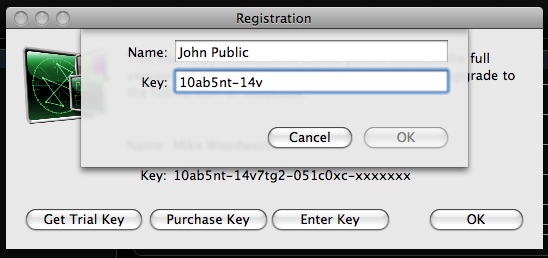
\includegraphics{images/registration.png}
\caption{Registration Window}
\end{figure}

\section{Updating}

ScopeBox automatically checks for updates during startup. If you'd like
to force it to check for an update, select ``Check for Updates'' from
the ScopeBox menu.

You can disable automatic updates via the ``General'' tab of the pref-
erences dialog.

\begin{quote}
\textbf{ScopeBox can only check for updates if you are currently
connected to the internet. If your ScopeBox system is not connected, you
can always download an updated copy from
\url{http://www.divergentmedia.com/scopebox}.}
\end{quote}

\chapter{Application Overview}

The main ScopeBox window can be broken into 4 distinct regions. These
are (a) the source bar at the top, (b) the palette region, (c) the
recorder and cliplist, and (d) the sidebar.

\begin{figure}[htbp]
\centering
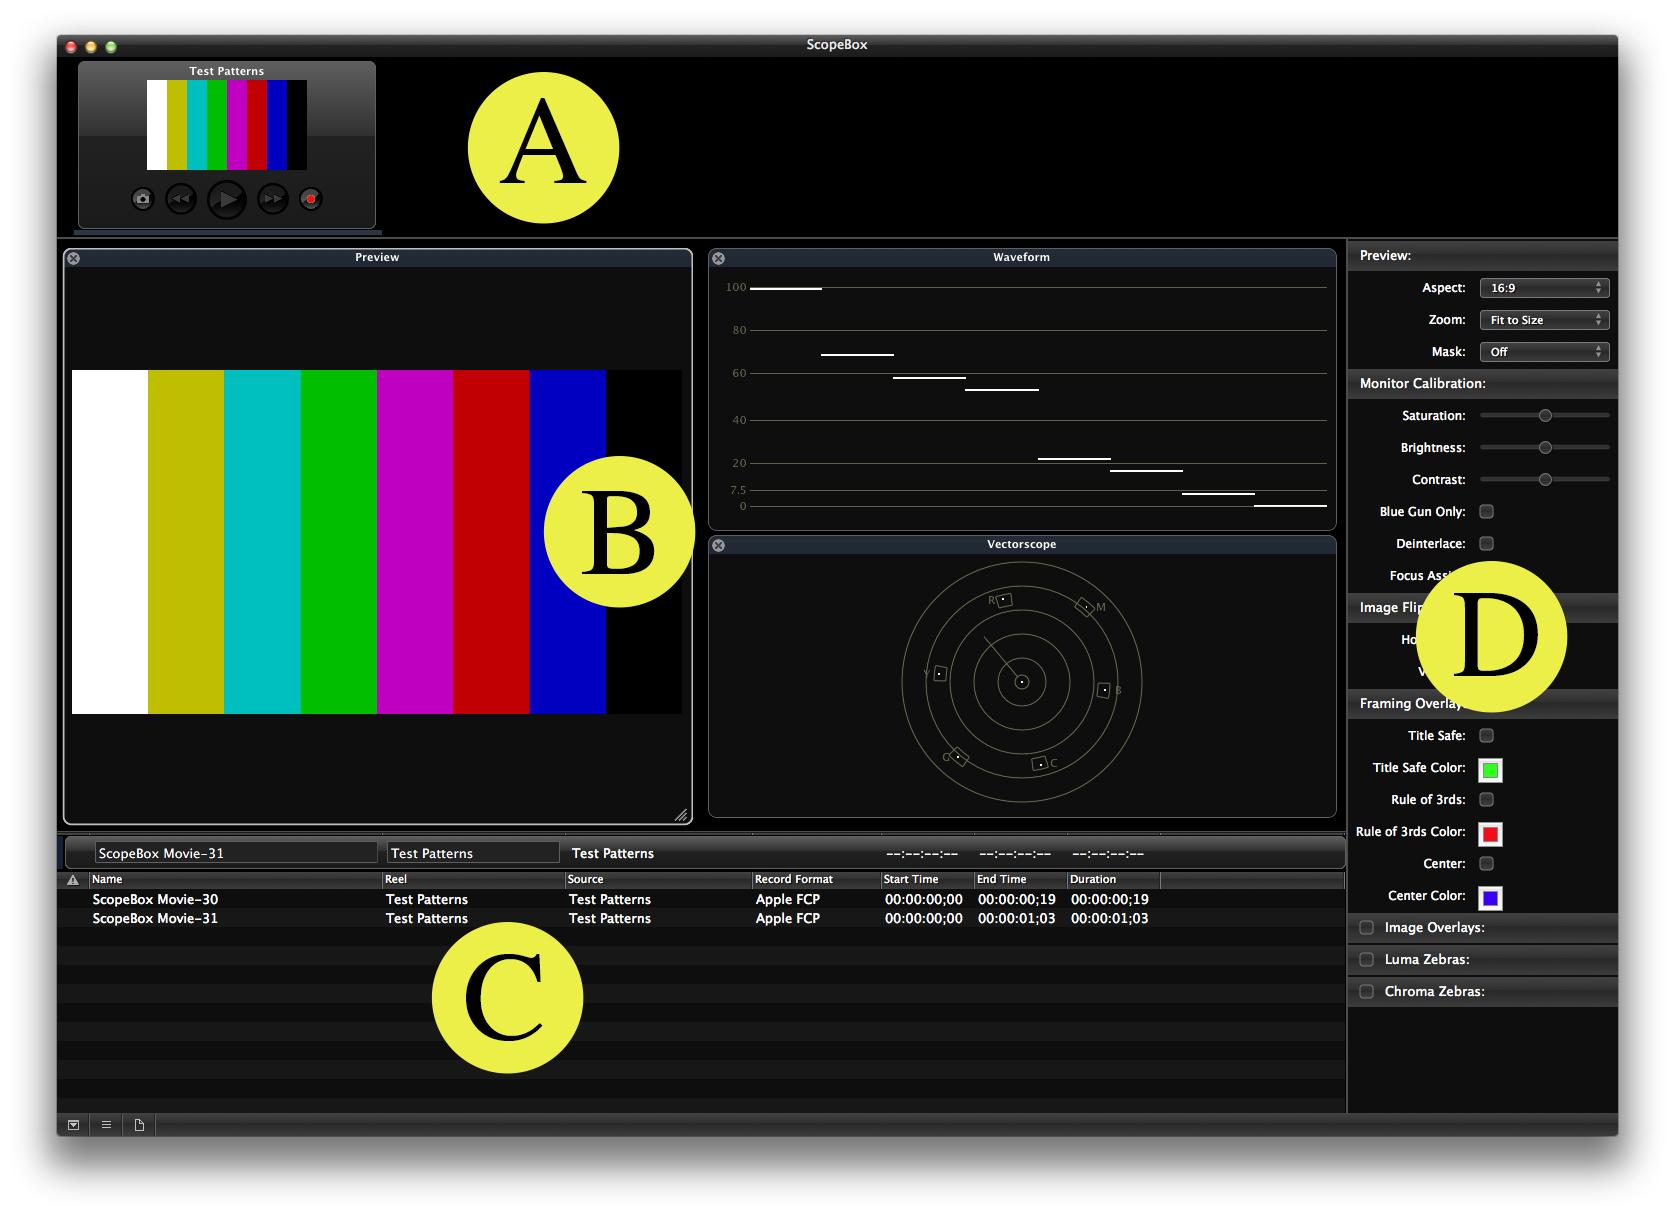
\includegraphics{images/MainWindowWithLabels.png}
\caption{A sample view of ScopeBox's main window.}
\end{figure}

\section{The Source Bar}

Each source you add appears in the source bar as a small preview with
built in VU meters, deck control buttons, still grabbing and recording
buttons. This preview is called the Source Palette.

You can mix and match any combination of source types. The num- ber of
devices that may be used simultaneously is limited only by the
processing power and bus bandwidth of your computer.

\section{The Palette Region}

Once you've added a source, you're free to start inspecting the signal
in a variety of ways. You do this by adding palettes to the source. Each
new palette you add will give you an additional tool to quanti- tatively
or qualitatively examine the video, audio, or timecode signal of that
source.

When a new palette is added, it appears in the Palette Region. This area
serves as your general workspace for analyzing sources. You can add or
remove palettes, change the source they monitor, or alter their size and
position at any time.

\section{The Sidebar}

Changing the settings of one of your sources or palettes is done in the
sidebar. Clicking on a palette, source, or recorder (which we'll get to
in the next section) will select it. You can tell which item in the
window is selected by the bright white border drawn around it. When an
object is selected, a number of controls will appear in the sidebar.
Changing these settings will alter the behavior of the selected object.

\section{The Recorder and Clip List}

If you're upgrading from ScopeBox 2.0, you may notice that the Re-
corder is no longer displayed when you add a new source. Instead, it is
available when you reveal the Clip List. This gives you more space for
your palettes, and access to all of your recordings is only one click
away.

\begin{figure}[htbp]
\centering
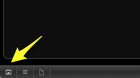
\includegraphics{images/cliplistToggle.png}
\caption{Reveal the ClipList}
\end{figure}

To reveal the Recorder and Clip List, click the icon in the lower left
corner of the window. You'll see a bar for each source. This is your
recorder settings bar. It works in tandem with the record button in the
source palette to allow you to set up video and audio records, as well
as get feedback for records currently happening. You'll see a separate
color-coded recorder settings bar for each recordable source currently
open.

The recorder settings bar has fields for the name of each file to be re-
corded, the reel info embedded in QuickTime movies, and the start time,
end time and current duration of any recordings in progress. In
addition, clicking on the bar reveals the in-depth settings for each
recorder.

Beneath this is the cliplist. This list allows you to review at a glance
all the day's prior recordings, and change names or reel info.

You can toggle to a thumbnail view of your recordings using the sec- ond
icon from the left, which looks like a series of horizontal lines.

\begin{figure}[htbp]
\centering
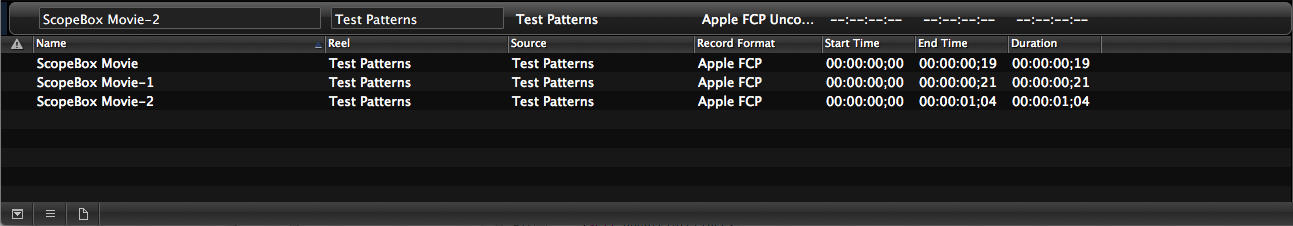
\includegraphics{images/cliplist.png}
\caption{List View}
\end{figure}

\begin{figure}[htbp]
\centering
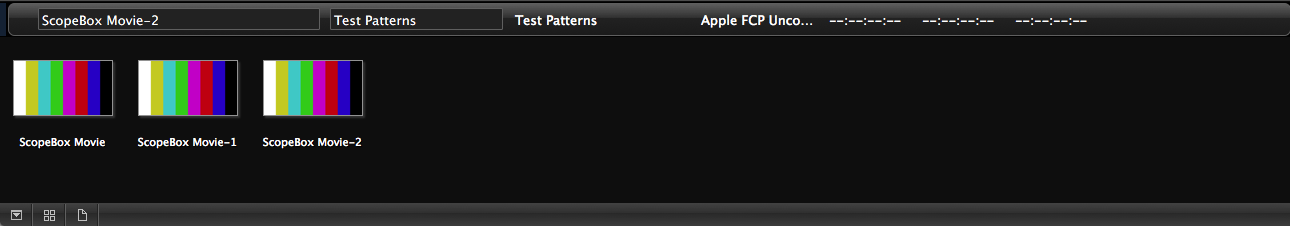
\includegraphics{images/thumblist.png}
\caption{Thumbnail View}
\end{figure}

\chapter{Dealing with Sources}

\section{Adding a Source}

The Source menu allows you to add new sources. In addition, new sources
can be added by right clicking within the source bar and choosing the
desired source under Add Source.

\begin{figure}[htbp]
\centering
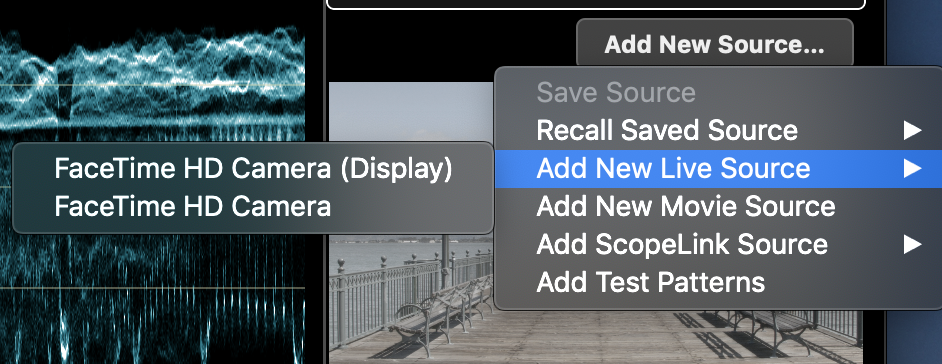
\includegraphics{images/AddingSource.png}
\caption{Opening a new source from the Source menu.}
\end{figure}

By default, you will be presented with the options ``Add Live Source''
and ``Add Movie Source.'' You may see additional sources, depending on
installed plug-ins. All standard FireWire cameras and Quick- Time
compatible capture cards will appear under the ``Add Live Source'' menu.

The ``Movie Source'' menu allows you to open any QuickTime-com- patible
video within ScopeBox.

\subsection{Unavailable Sources}

If a source is unavailable, it will be grayed-out in the menu. A source
may be unavailable for many reasons:

\begin{itemize}
\itemsep1pt\parskip0pt\parsep0pt
\item
  It is already open in ScopeBox or another application.
\item
  Your system is missing the necessary codecs or drivers.
\item
  There is a conflict between devices on your FireWire bus.
\end{itemize}

If you are having problems with a device please refer to the source
diagnostics and troubleshooting sections near the end of this manual.

\section{Removing a Source}

To remove a source, simply select the source's palette in the source
bar, and choose ``Remove Source'' from the Source menu. You can also
right click on a Source Palette and choose ``Remove Source''.

\begin{figure}[htbp]
\centering
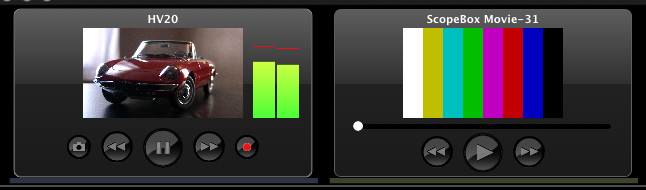
\includegraphics{images/DualSources.png}
\caption{Examples of the live source (left) and QuickTime source (right)
Source Palettes.}
\end{figure}

\section{The Source Palette}

Once you've added a source, its Source Palette will appear in the source
bar at the top of the ScopeBox window. The source palette is a quick way
to confirm you are receiving the proper video and audio signals. Below
the video preview, you'll find a set of controls for either deck control
or movie shuttling. If the source is recordable, buttons will be
available for grabbing a still and starting and stop- ping records.

\section{Changing a Source's Settings}

If you click on the preview palette, the left side of the window will
display all the appropriate options for that source. These will depend
upon the type of source you have selected.

Settings are split into three sections: video, audio and time- code.
Unchecking the checkbox next to any of these will disable that channel
of the source.

\subsection{Video}

You may change the name of the source using the Device field - just
click and begin typing. This can be useful when using more than one of
the same device.

The ``Input'' dropdown allows you to select which input you would like
assigned to this source. This dropdown will only show up for devices or
capture cards with multiple inputs. However, many such devices choose to
present themselves as discrete devices rather than a single source with
different inputs. In those cases, the dropdown will be disabled, and
you'll select the input as part of the device selection process.

\begin{figure}[htbp]
\centering
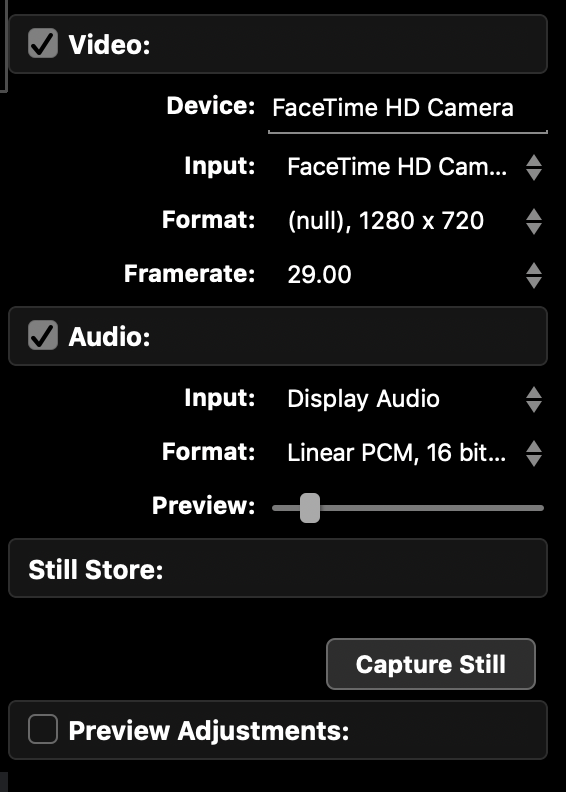
\includegraphics{images/SourceSidebar.png}
\caption{The source setting sidebar for an HDV Camera}
\end{figure}

The ``Compressor'' dropdown allows you to change the compression scheme
used to display and record the source. ScopeBox will convert your video
to the selected format in realtime. By default, this box will reflect
the native format of your source. Keep in mind that compression can be
very CPU-intensive.

\begin{quote}
\textbf{This isn't the area to change your record format. See chapter 17
for details on transcoding during record.}
\end{quote}

The ``Preview Level'' dropdown allows you to change the quality level
ScopeBox uses to decompress your video before processing and dis-
playing it. By default this will be set to High, and can be left alone
unless your machine is unable to process your current source at full
resolution without dropping frames.

The ``Setup'' dropdown allows you to change the setup level of your
video. This is the baseline level for black in your video. You shouldn't
change this setting unless your black levels appear to be incorrect in
the waveform palette. Additionally, before altering this setting, be
sure that your capture card drive is properly configured. This setting
will not impact recordings.

If your device presents custom controls to QuickTime the advanced
settings button allows you make adjustments to these.

HDV FireWire devices will have a checkbox to enable I-Frame only
decompression. This only decompresses every twelfth to fifteenth frame,
allowing HDV to be used with much older or slower ma- chines that might
not otherwise be able to process HDV video. Due to the nature of HDV
video, I-Frame only decompression allows the frames that do arrive to be
displayed with much lower latency as well.

DV and DVCProHD FireWire devices will have a ``Remove Dupli- cate
Frames'' checkbox. If your camera supports pulled up progres- sive
formats, this allows you to strip any duplicate frames from the signal,
and record a progressive movie, without wasting the disk space on
redundant frames.

Currently ScopeBox can properly process duplicate frames in:

\begin{itemize}
\itemsep1pt\parskip0pt\parsep0pt
\item
  DV24pA
\item
  DVCproHD 720p24
\item
  DVCproHD 720p30
\item
  DVCProHD 1080 24pA
\end{itemize}

\begin{quote}
\textbf{When using dupe re- moval with DVCProHD cameras such as
Panasonic's HVX200, it is important to choose the correct format in the
camera's menus. See the troubleshooting and source diagnostics sections
near the end of this manual for more information.}
\end{quote}

\subsection{Audio}

The audio section allows you to select an audio source for record- ing
and adjust the level at which the audio is played through your computer
speakers.

The preview audio adjustment is for monitoring only - any changes you
need to make to adjust the levels you see within your VU meters should
be done in your camera's audio controls.

\subsection{Timecode}

If your device is connected via FireWire and supports AVC protocols (DV,
DVCProHD, or HDV devices) then timecode and deckcontrol will
automatically be activated and configured. If you are using any other
device, you will see a popup to choose a serial port for connect- ing to
decks or cameras via Sony rs232/rs422 protocol.

Because serial deck control does not provide information about the
timecode format of the device, you'll also need to choose the appro-
priate timecode format to tag incoming timecode.

\subsection{Preview Adjustments}

It's often helpful to preview a signal with adjustments applied, to get
a sense of how an image will look after color correction is applied or
other changes are made. For example, when shooting in the log space, you
may wish to preview the image in the linear space. The Preview
Adjustments section of the source settings allow you to ap- ply these
adjustments via LUTs (look up tables)

ScopeBox supports two LUT formats, cube (1d and 3d) and 3dl. To apply a
LUT, check the Preview Adjustments box and then click Set Path. This
will allow you to load a LUT in one of the supported formats. You may
easily toggle the LUT on and off by checking the Preview Adjustments
box.

LUTs impact all of the palettes, including the preview and any scopes.
LUTs \textbf{do not} impact recorded files. LUTs are automatically
reloaded if they contents of the LUT file changes on disk.

\section{Drop Frame Warnings}

Periodically, under high usage you may see a yellow caution icon ap-
pear next to the video preview in the source palette. This is ScopeBox's
warning that the source has dropped one or more frames. You can reset
this warning by right-clicking on the source palette and choosing
``Reset Drop Frame Warnings.''

\begin{figure}[htbp]
\centering
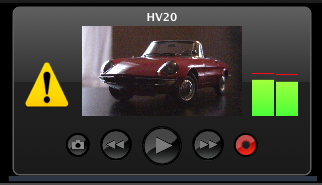
\includegraphics{images/DroppedFrame.png}
\caption{A Source Palette showing the dropped frame warning icon.}
\end{figure}

While a certain number of dropped frames are unavoidable under
conditions of extreme system usage, it's also possible to see dropped
frames when adding or removing sources. If the drop frame warn- ings are
persistent, check the performance section near the end of this manual
for tips on diagnosing the problem.

\section{Saving and Recalling Sources}

Once you've adjusted all of your source settings, you can save a preset.
Highlight the source in the source bar, and then select ``Save'' from
the Source menu. This will save all of the settings for the source,
including recorder settings and alerts.

\begin{figure}[htbp]
\centering
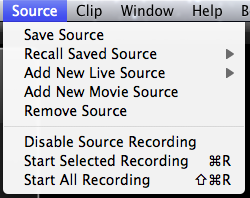
\includegraphics{images/saveSource.png}
\caption{Saving a Source}
\end{figure}

To recall a source, select it from the ``Recall Saved Source'' menu.

Sources will be saved with the device name set in the sidebar (see
above).

You can set a default source, which will automatically be loaded (if
available) when ScopeBox is launched, in the preferences.

\chapter{Palette Overview}

\section{Working with Palettes}

ScopeBox displays all content in flexible palettes within the palette
region of the ScopeBox window. The settings for each palette are
displayed in the sidebar on the right side of the ScopeBox window
whenever a palette is selected.

You may add multiple copies of each palette, each with its own set-
tings. For example, you may choose to open a preview palette for each of
your sources, and you may choose to also multiple preview palettes for a
single source, each with distinct settings.

\begin{figure}[htbp]
\centering
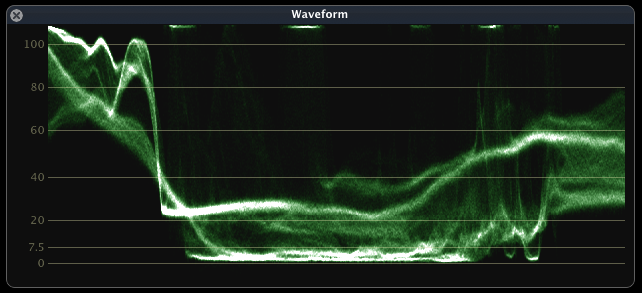
\includegraphics{images/waveform.png}
\caption{A standard palette in ScopeBox}
\end{figure}

\subsection{Adding Palettes}

To add new palettes, select the desired palette type from the Palettes
menu or right click on the background of the ScopeBox window or on the
source palette.

\subsection{Closing Palettes}

To close a palette, click the ``x'' in the upper left corner or hit the
De- lete key while the palette is selected. You may also right click
palette and select ``close.''

\subsection{Moving Palettes}

Click and drag to move a palette to the desired position. You can also
use the arrows keys for very precise positioning of a selected palette.

\begin{figure}[htbp]
\centering
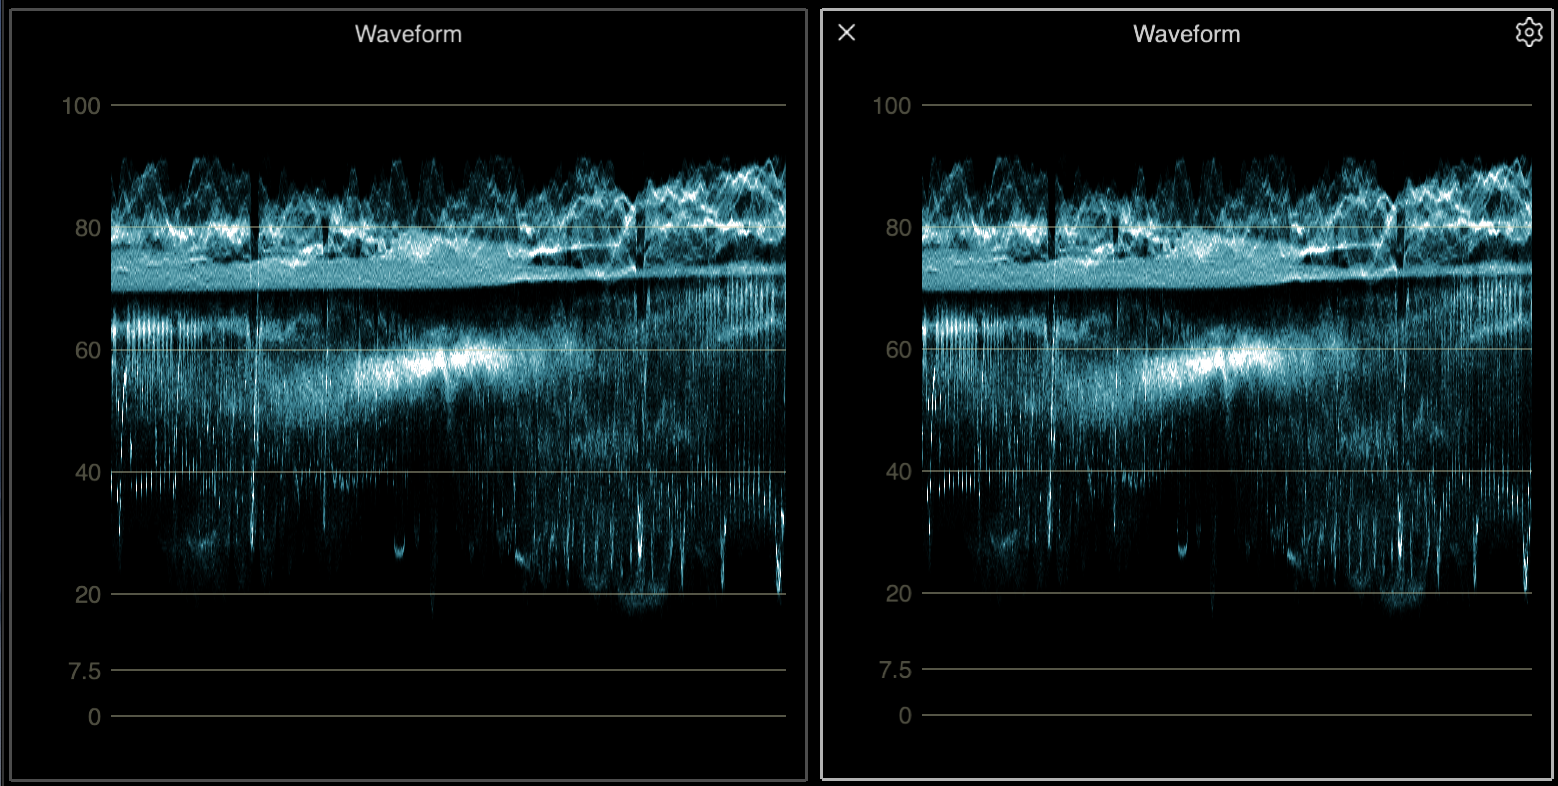
\includegraphics{images/DualWave.png}
\caption{A waveform palette unselected (left) and selected (right)}
\end{figure}

If you wish to organize your palettes with more precision, you can
``Enable Snapping'' in the Layouts menu. This will constrain your
palette's movement and re-sizing to an internal grid, allowing you to
easily line up multiple palettes.

\subsection{Resizing Palettes}

Click and drag on the lower right corner to resize a palette.

\subsection{Soloing Palettes}

Soloing a palette allows you to temporarily hide all other palettes and
focus your attention on the selected palette re-sized full screen. You
can activate a palette's soloing by choosing Solo Palette from the View
menu, by right clicking on the palettes.

\subsection{Open in New Window}

While ScopeBox defaults to a ``one-window'' view, you can extract any
palette into its own window. This makes it easy to use Scope- Box in a
multi-monitor configuration. To open a palette in its own window, right
click on the palette and select ``Open in New Win- dow.'' To view the
settings for a windowed palette, right click on the palette and select
``Show Palette Settings.''

\subsection{Switching Sources}

When you have multiple source open, each palette contains a set of small
circular buttons in the upper right corner. Each button cor- responds to
a source in your Source bar. To select which source the palette is
monitoring, click the button corresponding to the desired source's
color.

You can also change a palette's source by right clicking and choosing a
new source from the Source sub-menu.

\section{Common Settings}

Some settings are shared among many palettes. They are detailed in this
section.

\subsection{Sampling}

By default, ScopeBox scopes process video at full resolution, which may
be too resource intensive for slower computers or high defini- tion
signals. Selecting a sub-sampling multiplier tells the scope to look at
only every other line (2), every fourth line (4), or every eighth line
(8) when computing the scope.

\subsection{Intensity}

When in weighted mode, the intensity slider adjusts the brightness of
the scope. By changing this value, you adjust the visibility of areas of
low pixel concentration.

\subsection{Colors}

The color of the graticules and traces can be set in the application
preferences, available under the ``ScopeBox'' menu.

\chapter{Preview Palette}

The Preview palette displays video source output and can replace a
traditional field monitor for checking focus, framing, and color
calibration.

\begin{figure}[htbp]
\centering
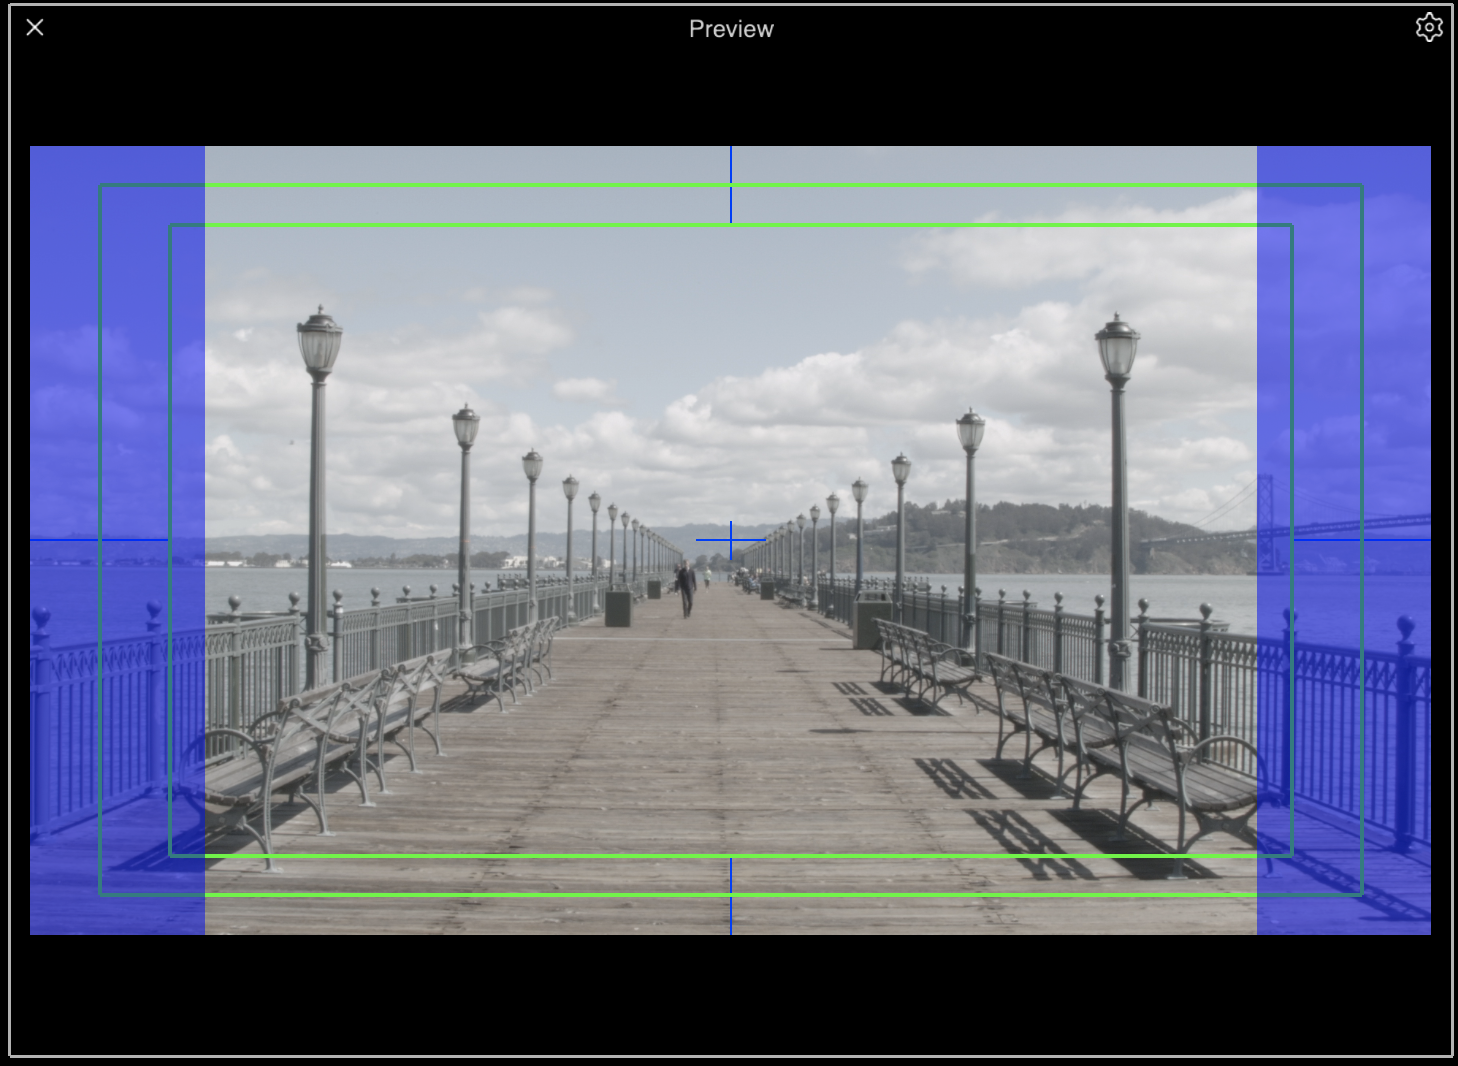
\includegraphics{images/PreviewWithOverlays.png}
\caption{The Preview Palette with 4x3 mask, center marks, and title safe
overlays enabled.}
\end{figure}

\section{Controls}

When you select the preview palette, the following controls will ap-
pear in the sidebar.

\begin{quote}
\textbf{Changes made to the image in monitor calibration only affect
what you see in the preview palette. They are not reflected in any other
scopes, nor are they recorded to disk. Monitor Calibration should only
be used to ensure your preview accurately reflects the video signal. You
can do this by calibrating to color bars sent from your source device.}
\end{quote}

\subsection{Aspect}

Controls the aspect ratio at which the video source will be displayed.

Standard Definition video uses rectangular pixels whereas computer
monitors use square pixels. This can result in video images that are
stretched when displayed on a computer. If you're shooting HD, the 16:9
option should be selected by default. For SD sources, you can either
view the native ``rectangular'' pixels, or the corrected ``square''
display. When you choose a new source, ScopeBox will automati- cally set
your preview's aspect to match that of the incoming image.

\subsection{Zoom}

Zoom sets the size of your image. 100\% and 200\% set the video image to
the corresponding magnification no matter the size of the preview
palette. This gives you a pixel-for-pixel view of your image with no
interpolation from the graphics card or video re-size, which is
especially useful when trying to set focus. However, if your palette is
too small you may not see the whole image. ``Fit to Size'' fits the
video to fill the palette, but does so by re-sizing the image which may
introduce minor sub-sampling interpolation - leading to a slightly
blurrier image.

\subsection{Mask}

The mask overlay draws blue bars as a framing guide when shooting at an
aspect ratio other than the destination ratio. Using this will allow you
to frame shots not only for the acquisition format, but for any other
formats you may have to deliver to as well. For instance, if you know
the video you are shooting in HD (16x9) will be used in an SD
production, setting your mask to 4x3 will allow to see where by default
the image will be cropped in the format change.

\subsection{Monitor Calibration}

The Saturation, Brightness, and Contrast sliders provide simple cor-
rection of the Preview image. These corrections are used to compen- sate
for differences in computer monitors. Calibrating the Preview palette
ensures that the image accurately represents what the camera is
shooting. Any changes made do not affect the video captured to disk or
the video monitored in any other scope.

\subsection{Blue Gun}

When checked, the Preview palette displays the blue channel as black and
white, ignoring red and green. This simulates the ``blue only'' button
on many CRT monitors, which is useful when calibrat- ing a monitor with
SMPTE color bars.

\subsection{Flip}

Flips the preview image horizontal and/or vertically. This function can
be used to correct for a lens adapter or 3d rig that flips the image.

\subsection{Deinterlace}

Deinterlace blends the two frames of an interlaced source together. This
will remove the ``comb'' effect which can appear when viewing interlaced
video on a progressive monitor.

\subsection{Focus Assist}

Focus Assist is similar to the ``peaking'' feature found on some cam-
corders. This will add highlights to your video at sharp edges. This can
be helpful when adjusting focus.

\subsection{Title Safe}

Title Safe adds two overlay boxes to the video. The outer box shows the
graphics safe region and the inner box shows the title safe region. Make
sure important action happens inside the title safe box, as older
televisions may crop beyond it.

\subsection{Rule of Thirds}

Provides a 3x3 grid to assist with composition.

\subsection{Center}

Provides center cross-hairs to assist with composition.

\subsection{Luma Zebra}

Luma Zebra overlays rolling stripes on the brightest areas of the im-
age. These areas may be overexposed. The slider controls the thresh-
hold at which the zebras appear. The stripe color is displayed in the
square to the right and can be clicked to select another color.

\subsection{Chroma Zebra}

Chroma Zebra is similar to the Luma Zebras but overlays a zebra pattern
on the areas of highest saturation.

\subsection{Overlay}

Overlays allow you to open an image or QuickTime movie to super- impose
on top of you live video. These images can be custom guides for framing
around your productions lower thirds, a background that will later be
chroma keyed into the shot, or video footage you need to match framing
or exposure in.

To add an image, make sure the dropdown is set to ``Custom Image'', and
drag and drop an image into the image well below. In addition, any other
open movie or live source can be selected from the drop- down to use it
as the superimposed item. Below the image well is a slider to adjust the
opacity of the overlay.

\chapter{Audio Meters}

The Audio Meter displays the level of the audio signal in dBFS. It
provides both an instant meter and an averaging peak meter. Every spike
is displayed, even if very brief.

\begin{figure}[htbp]
\centering
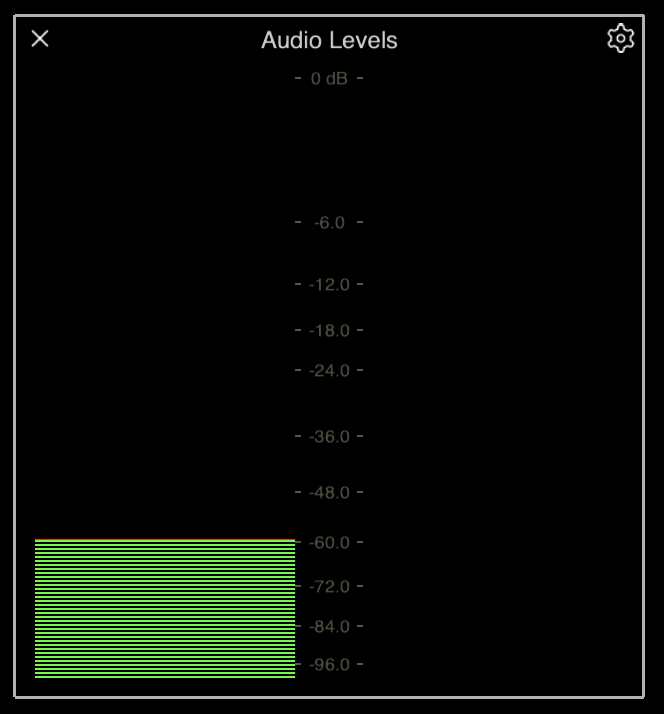
\includegraphics{images/AudioLevels.png}
\caption{The Audio Meter Palette}
\end{figure}

\section{Controls}

\subsection{Channel Count}

By default the Audio Meter will show all channels currently reported by
a source. However, many devices report a fixed number of output
channels, which can waste valuable screen space displaying empty
channels. If you're shooting with a camera that sends eight channels to
ScopeBox, but are only using two, you can set channel count to 2 to only
present the first two channels.

\subsection{Scale}

Different source formats require different peak audio levels. This level
is often referred to as Unity. When working with bars and tone, or when
trying to set your mic volumes at the proper levels, you want to know
exactly where unity lies in the Audio Meter. ScopeBox pro- vides a set
of Scale markers for each of the three major unity levels found on
professional video devices -12, -14 and -20 dB.

\chapter{Surround Meters}

The Surround Meters give you a way to visualize your audio signal in a
surround sound context. This allows you to quickly analyze the surround
components of your audio mix, even in environments that don't lend
themselves to proper audio monitoring.

\begin{figure}[htbp]
\centering
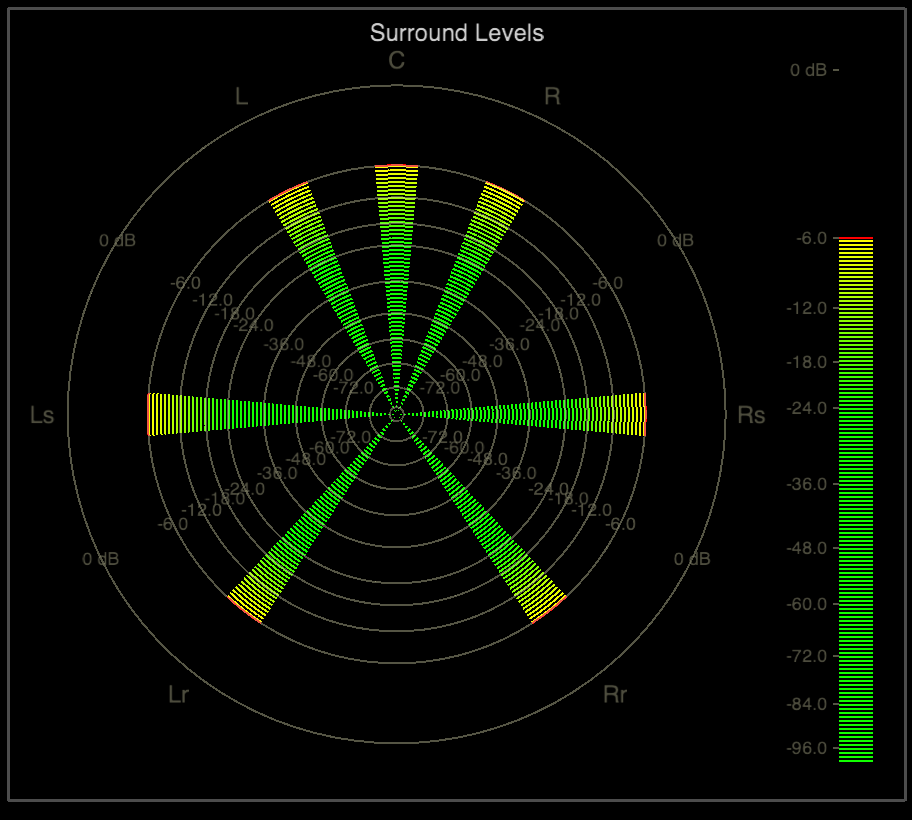
\includegraphics{images/SurroundLevels.png}
\caption{The Surround Meter Palette}
\end{figure}

Because audio inputs do not inherently pass information about how to lay
out each channel in a surround environment, ScopeBox pro- vides a
variety of popular channel layouts. Select the layout which matches the
input layout you are feeding ScopeBox.

The palette settings also allow you to set the scale, and enable a
``peak hold'' option, similar to the Audio Meters (see
\hyperref[Audio-Meters]{section 7}).

\chapter{Waveform}

The Waveform scope provides a view of the luminance in the video signal.
The vertical axis corresponds to luminance while the horizon- tal axis
matches the horizontal axis of the video source.

\begin{figure}[htbp]
\centering
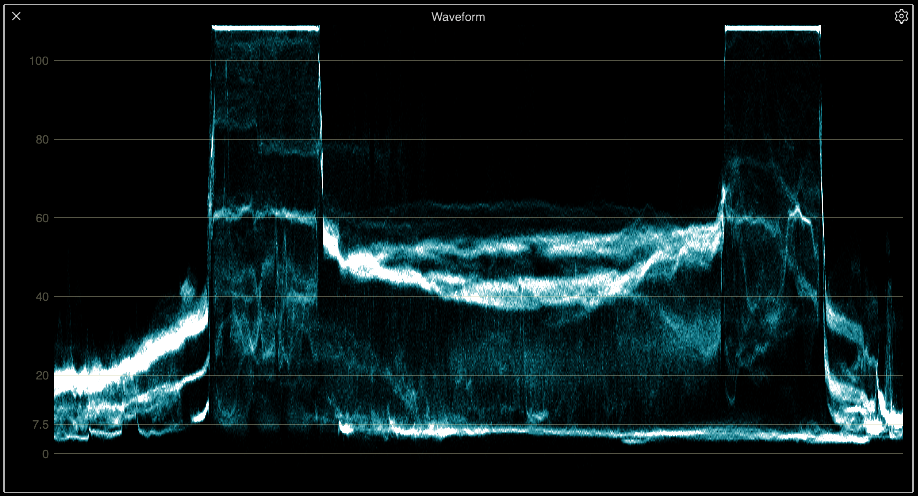
\includegraphics{images/waveform-wide.png}
\caption{The Waveform Palette}
\end{figure}

\section{Controls}

\subsection{Mode}

The Mode dropdown allows you to choose the method ScopeBox uses to
render your scope. Each mode offers you different informa- tion:

\emph{Weighted} mode looks more like a traditional raster scope and
express- es the number of pixels at a given value by varying the
brightness.

\emph{Mono} displays every data point at full intensity, which can be
useful in ensuring complete legality. With weighted views it is possible
to miss a small pixel region that is out of range.

\emph{Colorize} replaces the traditional green in a scope and with the
actual color that it represents. For example, if someone is wearing a
bright red shirt, there will be a bright red streak where the scope
renders those pixels.

\subsection{Filter}

The Filter dropdown allows you to select between the three com- monly
found filter types found on hardware waveform monitors - \emph{Luma},
\emph{Chroma} and \emph{Flat}. Luma is the default, causing the waveform
to display only the luminance (Y) channel of your video. Chroma will
display only the chrominance (C) channel of your video. Flat combines
the two channels, and gives you a view of the total overall levels
within your video. Flat and Chroma will always use NTSC I/Q scaling.

\subsection{Instantaneous Envelopes}

Instantaneous Envelopes help ensure that you don't miss any data within
your waveform monitor, even when it's just a single pixel. Checking the
box will cause two bounding lines to be added to your waveform, one
showing the maximum values for your waveform, and one showing the
minimum values for each vertical line.

\subsection{Peak Envelopes}

Peak envelopes show the maximum and minimum values for your waveform
over time. This allows you to look away from your scopes, and still know
whether you exceeded a target threshold. The reset button will clear the
peak values.

\subsection{Scale}

There are four different Scale options available for measuring your
waveform. These are IRE (the traditional scale for a waveform monitor),
8 bit, 10 bit and mV (millivolt). The 8 bit and 10 bit op- tions allow
you to measure your waveform according to the actual sample values in
the signal. Millivolt allows you to compare against the signal shown by
a traditional hardware waveform monitor or oscilloscope.

\chapter{Vectorscope}

The Vectorscope displays chrominance (color) information. Satu- ration
is indicated by distance from the center while the position around the
circle indicates hue.

\begin{figure}[htbp]
\centering
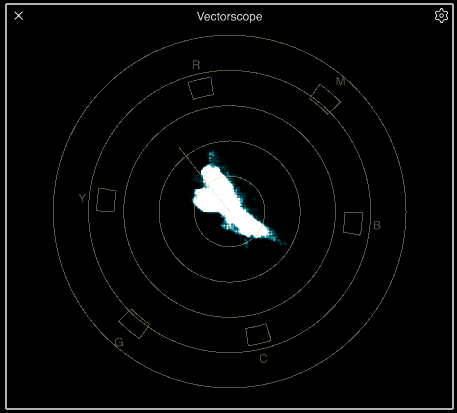
\includegraphics{images/vectorscope.png}
\caption{The Vectorscope Palette}
\end{figure}

The markers on the Vectorscope (R, Y, B, etc) indicate colors. The boxes
show where the signal should land when displaying the stan- dard SMPTE
color bars signal, providing a guide for gauging satura- tion. The
targets are plus and minus 5 degrees and 5\% saturation.

The rings represent saturation percentage, in 20\% increments (the in-
nermost circle represents 20\% saturation, the next 40\%, etc).

\section{Controls}

\subsection{Colorspace}

The colorspace option provides three different colorspaces with which to
view the vectorscope. These are NTSC, Rec. 601 and Rec. 709. By default,
ScopeBox will automatically set the colorspace based on your source.
These colorspaces will adjust the color targets and scaling of the
vectorscope.

\subsection{Mode}

The Mode dropdown allows you to choose the method ScopeBox uses to
render your scope. Each mode offers you different informa- tion:

\emph{Weighted} mode looks like a traditional scope and expresses the
num- ber of pixels at a given value by varying the brightness.
\emph{Mono} mode displays every data point at full intensity, which can
be useful in ensuring complete legality. With weighted views it is pos-
sible to miss a small pixel region that is out of range. \emph{Colorize}
mode replaces the traditional green in a scope and with the actual color
that it represents. For example, if someone is wearing a bright red
shirt, there will be a bright red streak where the scope renders those
pixels.

\subsection{Instantaneous Envelopes}

Instantaneous Envelopes help ensure that you don't miss any data within
your vectorscope, even when it's just a single pixel. Checking the box
will cause draw a boundary around the maximum values of your
vectorscope.

\subsection{Peak Envelopes}

Peak envelopes show the maximum and minimum values for your vectorscope
over time. This allows you to look away from your scopes, and still know
whether you exceeded a target threshold. The reset button will clear the
peak values.

\subsection{Hue Line}

The Hue Line can be thought of as a configurable target line. After
enabling this option, you can click and drag the hue line to place it at
any point on the vectorscope. You can also use the ``hue'' and ``power''
sliders to alter the line. This gives you a convenient reference mark
for color correction or matching shots.

\subsection{Flesh Line}

The Flesh Line is an industry standard reference line along which skin
tones will generally fall. It's most useful as a static reference
between scenes or cameras.

\subsection{Grat Style}

The default graticule style for the vectorscope a standard set of con-
centric circles, representing saturation. ScopeBox also offers a ``hue
vectors'' graticule style, which provides a more modern, color correct
and camera matching specific overlay. This view gives more contextual
information for hue adjustments across the entire range of saturations,
while removing unneeded clut- ter more appropriate for signal-analysis
and legality monitoring. The perpendicular hash marks on each line
represent a 75\% target

\begin{quote}
\textbf{Hue vectors graticule by
\href{http://vanhurkman.com/wordpress/?p=2563}{Alexis Van Hurkman} is
licensed under a
\href{http://creativecommons.org/licenses/by-sa/3.0/deed.en_US}{Creative
Commons Attribution-ShareAlike 3.0 Unported License}}
\end{quote}

\chapter{HML Balance}

The HML Balance palette can be thought of as three distinct vec-
torscopes, displaying information about the ``high,'' ``mid,'' and
``low'' components of your signal. This can be helpful for identifying
color casts in specific luminance regions of your image, like shadows or
highlights.

Because the crosspoints between the three vectorscopes are configu-
rable, this palette can be filtered in a variety of ways to allow you to
focus on just one component of your signal.

Many of the controls are similar to those found on the vectorscope, but
there are some HML-specific controls as well.

\begin{figure}[htbp]
\centering
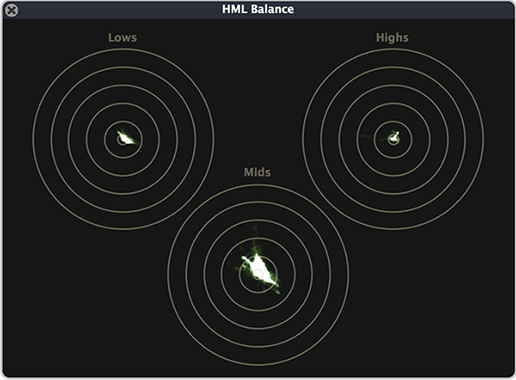
\includegraphics{images/HMLBalance.png}
\caption{The HML Balance Palette}
\end{figure}

\section{Controls}

\subsection{Zoom}

The Zoom control is a variable zoom, allowing you scale up the scopes to
see even the most minute detail. Keep in mind that with an 8-bit signal,
the amount of resolution available in the display is inherently very
limited.

\subsection{Luma Threshold}

The ``low'' and ``high'' values act as low- and high-pass filters,
respectively. Everything below the value entered in the ``low'' field
will be displayed on the low scope, everything above the value entered
in the ``high'' field will be displayed in the high scope, and
everything in between will be drawn in the mid scope.

\chapter{RGB Parade}

The RGB Parade displays individual waveforms for each channel (Red,
Green and Blue) of your video signal.

\begin{figure}[htbp]
\centering
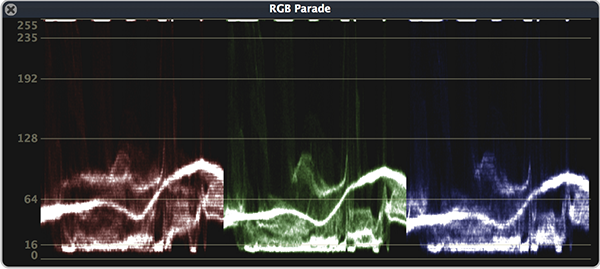
\includegraphics{images/RGBParade.png}
\caption{The RGB Parade Palette}
\end{figure}

You can use the RGB Parade to gauge separation between the color
channels. For example, when setting white balance, all three channels
should be equal horizontally, indicating that you have equal amounts of
red, green and blue, thus creating white.

The RGB Parade is also useful when trying to determine the cause of a
color cast in shadow or highlight areas. Such casts can be caused by
clipping (overexposure or underexposure) in one particular color
channel. It is often difficult to diagnose this issue without a special-
ized tool like the RGB Parade.

\section{Controls}

\subsection{Layout}

The layout control allows you to display your RGB parade as either
``R,G,B,'' ``B,G,R,'' or ``Overlay.'' Overlay mode will stack each chan-
nel, and composite their values.

\subsection{Mode}

The Mode dropdown allows you to choose the method ScopeBox uses to
render your scope. Each mode offers you different informa- tion:

\emph{Weighted} mode looks like a traditional scope and expresses the
num- ber of pixels at a given value by varying the brightness.

\emph{Mono} mode displays every data point at full intensity, which can
be useful in ensuring complete legality. With weighted views it is pos-
sible to miss a small pixel region that is out of range.

\subsection{Instantaneous Envelopes}

Instantaneous Envelopes help ensure that you don't miss any data within
your monitor, even when it's just a single pixel. Checking the box will
cause two bounding lines to be added to your waveform, one showing the
maximum values for your waveform, and one showing the minimum values for
each vertical line.

\subsection{Peak Envelopes}

Peak envelopes show the maximum and minimum values for each channel over
time. This allows you to look away from your scopes, and still know
whether you exceeded a target threshold. The reset button will clear the
peak values.

\subsection{Transform}

The transform allows you to control how a YUV source is converted to RGB
for monitoring.

\chapter{YUV Parade}

The YUV Parade displays individual waveform monitors for the Y, U and V
components of the signal.

\begin{figure}[htbp]
\centering
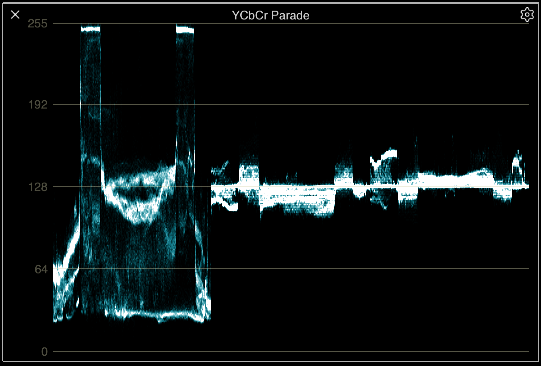
\includegraphics{images/YUVParade.png}
\caption{The YUV Parade Palette}
\end{figure}

The YUV Parade is useful for signal chain diagnosis since most video
devices process in the YUV colorspace.

\section{Controls}

\subsection{Mode}

The Mode dropdown allows you to choose the method ScopeBox uses to
render your scope. Each mode offers you different information.

\emph{Weighted} mode looks like a traditional scope and expresses the
num- ber of pixels at a given value by varying the brightness.

\emph{Mono} mode displays every data point at full intensity, which can
be useful in ensuring complete legality. With weighted views it is pos-
sible to miss a small pixel region that is out of range.

\subsection{Instantaneous Envelopes}

Instantaneous Envelopes help ensure that you don't miss any data within
your monitor, even when it's just a single pixel. Checking the box will
cause two bounding lines to be added to your waveform, one showing the
maximum values for your waveform, and one showing the minimum values for
each vertical line.

\subsection{Peak Envelopes}

Peak envelopes show the maximum and minimum values for each component
over time. This allows you to look away from your scopes, and still know
whether you exceeded a target threshold. The reset button will clear the
peak values.

\chapter{Luma Histogram}

The Luma Histogram displays the range of luminance levels in the video
signal, with black on the left and white on the right. The height of
each line corresponds to the percentage of the image that occurs at that
luminance level.

\begin{figure}[htbp]
\centering
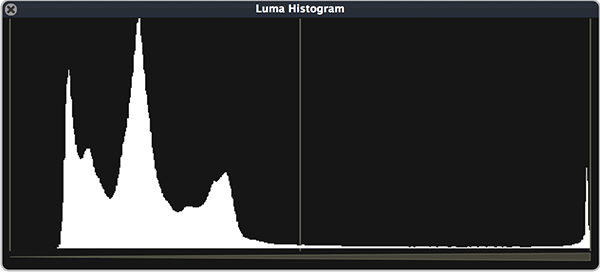
\includegraphics{images/LumaHistogram.png}
\caption{The Luma Histogram Palette}
\end{figure}

\section{Controls}

\subsection{Scaling}

The Luma Histogram can be toggled between ``log'' and ``linear''
scaling. In log mode, each horizontal graticule represents an order of
magnitude - 10, 100, 1000 and so on. This means that even lumi- nance
levels with relatively low frequency within your signal will be easily
visible within the palette.

Linear scaling causes the vertical axis to be scaled to the height of
the most populated luminance level.

\chapter{RGB Histogram}

The RGB Histogram displays the intensity of the Red, Green and Blue
signals. Similar to the Luma Histogram, the leftmost column is the
lowest intensity and the rightmost is the highest intensity.

\begin{figure}[htbp]
\centering
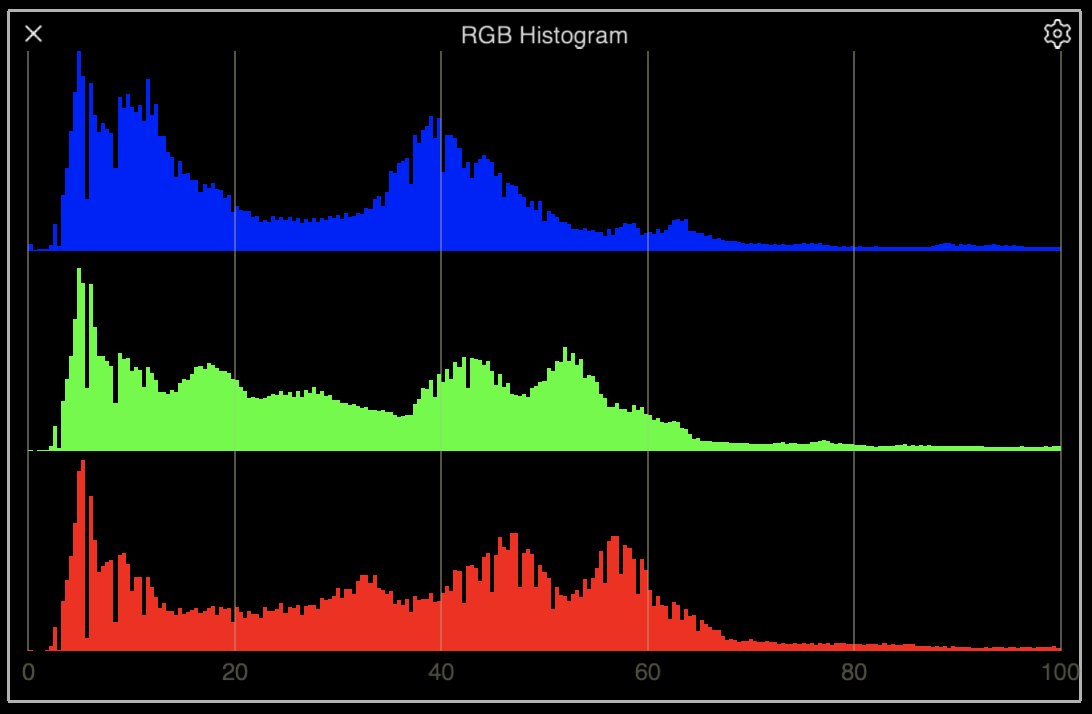
\includegraphics{images/RGBHistogram.png}
\caption{The RGB Histogram Palette}
\end{figure}

The RGB histogram is particularly useful when working with chroma key
shots. The key color should be as even as possible for clean keying.
Doing so produces a very tight clump of long bars rather than a wider
clump of short bars.

\section{Controls}

\subsection{RGB Transform}

The RGB Histogram provides a simple way to watch for gamut excursions.
The RGB Transform dropdown allows you to select from among three
transforms. This will draw vertical bars on the RGB histogram. Values
falling outsides these bars indicate a gamut excursion.

\subsection{Scaling}

The RGB Histogram can be toggled between ``log'' and ``linear'' scaling.
In log mode, each horizontal graticule represents an order of magnitude
- 10, 100, 1000 and so on. This means that even levels with relatively
low frequency within your signal will be easily visible within the
palette.

Linear scaling causes the vertical axis to be scaled to the height of
the most populated intensity for a given channel.

\chapter{Timecode}

The Timecode palette displays the timecode as sent from the video
source, generally when playing a tape or recording. Some devices operate
in ``free run'' mode, which generates timecode without a tape present.
Timecode is formatted in SMPTE standard format - Drop Frame timecodes
have a semicolon (;) between the seconds and frames place whereas Non
Drop Frame timecodes have a colon (:).

\begin{figure}[htbp]
\centering
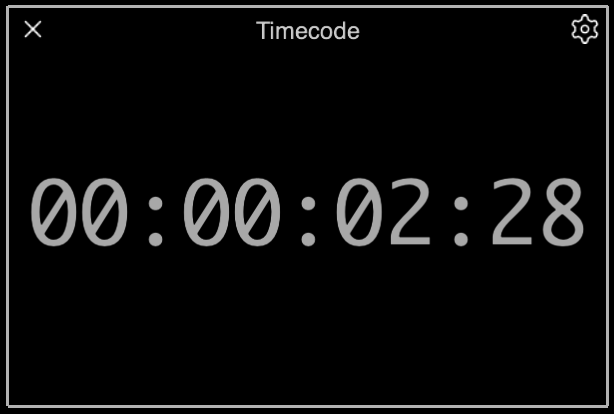
\includegraphics{images/Timecode.png}
\caption{The Timecode Palette}
\end{figure}

\chapter{Channel Plot}

The channel plot allows you to map two channels of a video signal on an
X/Y axis. The box drawn within the scope helps you deter- mine when your
signal will be clipped by a colorspace conversion (gammut errors).

\begin{figure}[htbp]
\centering
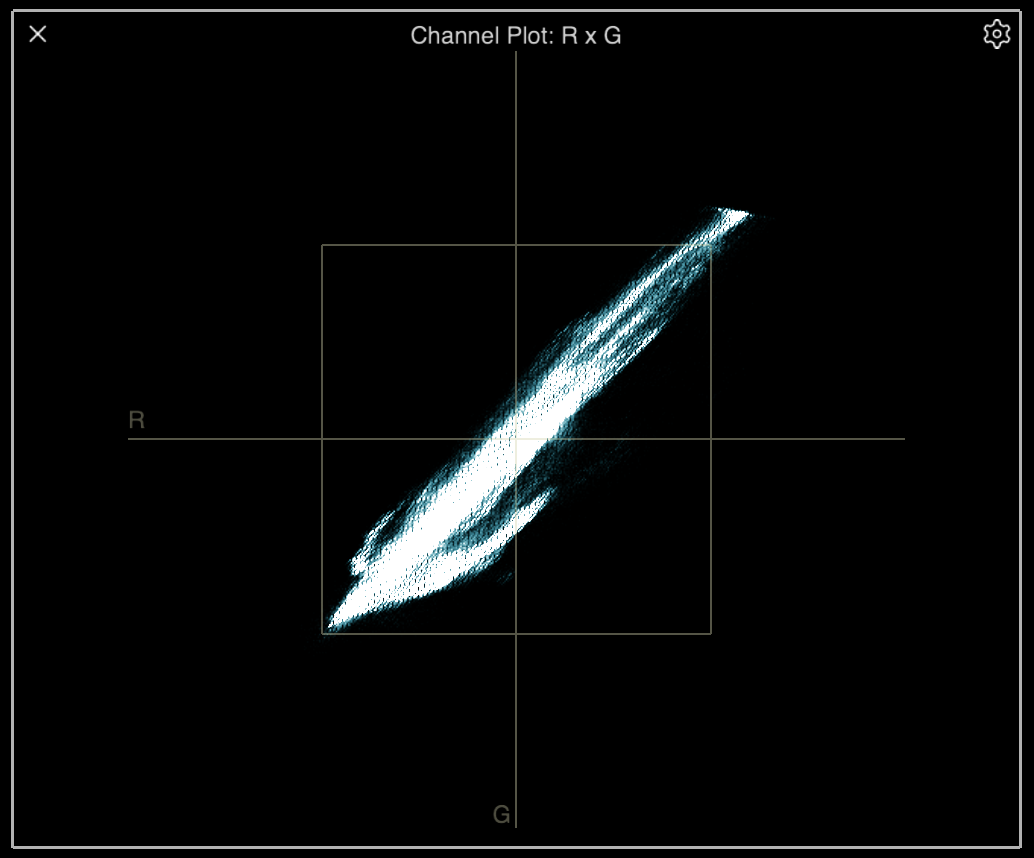
\includegraphics{images/ChannelPlot.png}
\caption{The Channel Plot Palette}
\end{figure}

\section{Controls}

\subsection{Axis Controls}

There are six different channels which may be plotted on either the X or
Y axis. These are Y, Cb, Cr and R,G,B. The channel plot is pri- marily
useful when plotting values within a single color format. For example,
you'd generally want to plot R against G or B, rather than against
Y,Cb,Cr. By plotting R versus G, and in a second palette, G versus B,
you'll be able to quickly judge whether any data will be clipped during
the YUV to RGB conversion.

\chapter{Quartz Composer}

Quartz Composer is an Apple technology for visually building graphical
compositions. ScopeBox allows you to use Quartz Com- poser projects as
plugins, to alter the display your video signal in realtime.

To load a Quartz Composer project, click the ``set path'' button and
browse to the QTZ file you wish to use. Quartz Composer projects dictate
which controls will be shown within the ScopeBox window.

If you save Quartz Composer projects (QTZ) in ScopeBox Appli- cation
Support folder (inside your Library folder) they'll appear as palettes
you can add to ScopeBox directly.

For details on creating ScopeBox-compatible Quartz Composer files, see
the separate ScopeBox 3 SDK documentation.

\chapter{Recording}

\section{Starting and Stopping a Record}

Each source has a record button, which can be used to stop and start
recording. By default, ScopeBox will store files in the location speci-
fied in your preferences. From the Source menu, you can also start
recording one or all of your sources simultaneously.

\begin{figure}[htbp]
\centering
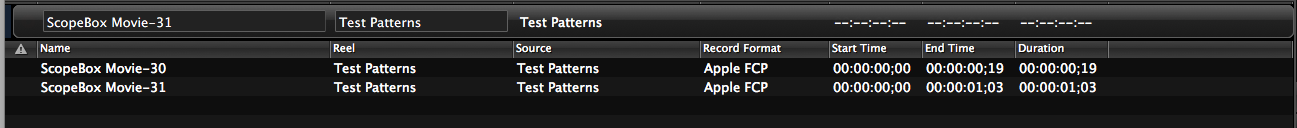
\includegraphics{images/RecordBar.png}
\caption{A recorder settings bar with cliplist below}
\end{figure}

\section{Recorder Settings Bars}

The name of the video file and the reel name are set for each record-
ing source in the source Recorder Settings Bar, which is revealed by
clicking the icon in the lower left corner of the ScopeBox window.

By clicking a source's Recorder Settings Bar, you can access addi-
tional options in the sidebar.

\begin{figure}[htbp]
\centering
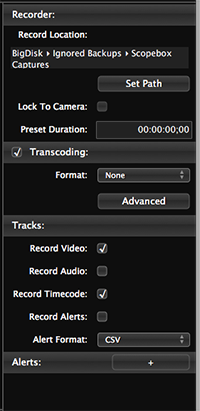
\includegraphics{images/RecorderSidebar.png}
\caption{Recorder Settings}
\end{figure}

\subsection{Record Path}

ScopeBox has a global record path setting (in the preferences win- dow).
In addition, you may set a record location on a per-recording basis
using the ``Set Path'' button.

Because multicam shoots can be disk-bandwidth intensive, spreading your
recordings across multiple drives may enhance performance.

\subsection{Lock to Camera}

When Lock to Camera is enabled, ScopeBox will monitor your attached
source's tape status. If the device goes into record mode, ScopeBox will
also begin to record. When the device returns to Stop or Pause state,
ScopeBox will stop the record. \textbf{Lock to Camera is not available
with devices connected via HDMI or HD-SDI.}

This allows you to easily record both on your camera and within ScopeBox
with one push of a button on your camera.

It's important to realize, however, that when Lock to Camera is en-
abled, the record button on your Source Palette will no longer work.
Lock to Camera also means that Scopebox will discontinue record- ing in
the event you run out of tape on your camera.

\begin{quote}
\textbf{Some cameras may not properly work with ScopeBox's Lock to
Camera feature. Specifically, many HDV cameras reset the timing
information in their video stream at the start of each recording. This
may cause Sco- peBox to record audio and video out of sync for the
remainder of that shot.}
\end{quote}

\subsection{Preset Duration}

If you'd like to utilize the LiveEdit functionality of ScopeBox, you'll
need to enter a preset duration for your recording. Make sure this
matches the length of the recording you intend to capture. By do- ing
this, you'll be able to import your recording into your editing software
and begin editing, while the capture is still in process. For maximum
compatibility, we would recommend keeping this value under four hours.
If you exceed this duration while editing, your record will continue,
but you'll need to manually reload your video in your editor to load new
content.

\subsection{Transcoding}

Transcoding allows you to convert your input source into another format
in realtime, during capture. If you're working with an un- compressed
source, this can be particularly helpful, allowing you to capture into a
modern, visually lossless format like ProRes or DNxHD. The format
dropdown provides a variety of presets for use with the major non-linear
editing platforms. Selections will be grayed out if the corresponding
codec is not available on your computer.

The advanced button allows you to create a custom transcoding set- ting.

Keep in mind that transcoding can be highly CPU intensive, particularly
with custom settings.. If you notice dropped frames or unacceptable
performance, you may wish to avoid using the trans- coding
functionality.

\subsection{Record Track Selections}

Sometimes you only need to record audio or video. In this case, un-
check any tracks you don't need, and Scopebox will omit them from any
future recordings - saving you disk space and CPU usage.

\subsection{Alerts}

Alerts allow you to set threshold values for your source, so that you
can know when an exception has occurred, even if you're not watch- ing
your screen at that exact moment. Alerts are explained in section 19.

\section{The Clip List}

The triangle in the bottom left of the window will open the Clip List
which shows you the history of all of your recordings. From the Clip
List, you can review previous shots, change their file names or reel
info, or check timecode information.

By right clicking on a clip in the Clip List, you can choose to open a
movie in QuickTime Player, to show the file in the finder, or to open
the clip as a new source in ScopeBox.

\subsection{Thumbnail Mode}

The button to the right of the show/hide Clip List button allows you to
toggle the Clip List between list mode and thumbnail mode. In thumbnail
mode you can easily see the first frame of each clip.

\section{Drop Frame Warnings}

If while you are recording, the source detects a dropped frame, a
warning will appear in both the Source palette and the associated
Recorder Settings Bar to alert you to the dropped frame in your recorded
clip.

The first column of the Clip List shows warnings for any previous clip
which experienced dropped frames or custom alerts, allowing you to
quickly review what may need to be reshot.

\section{FailSafe Recording}

ScopeBox 3 always writes coherent QuickTime files to disk. This means
that even if you experience some sort of interruption mid- recording (a
power outage, hardware or software failure, etc) the recording up to
that point will be playable. This feature is always active.

\chapter{Alerts}

Alerts provide a way to monitor your signal, even when you don't have
your eyes glued to the screen. Alerts are tied to recorders, and are
enabled on a source by source basis.

\section{Activating Alerts}

Alerts can be attached to any recorder. After revealing the cliplist,
click the recorder bar and check the box in the ``Record Alerts'' sec-
tion of the bar on the right.

You may also select a format for alert recording. In addition to
displaying in the cliplist, alerts will be saved to a file alongside
your recorded output. See the ``Export Formats'' section below for
details.

\section{Adding Alerts}

Initially, there are no alerts attached to your source. To attach
alerts, check the ``Record Alerts'' box and then click the ``add alert''
button and select an alert type.

\begin{figure}[htbp]
\centering
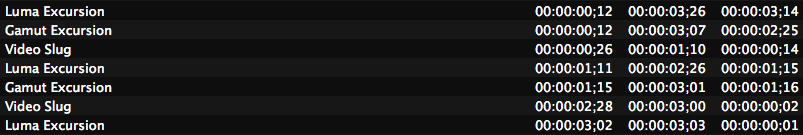
\includegraphics{images/alertList.png}
\caption{Alert List}
\end{figure}

\section{Alert Types}

Alerts generally consist of a threshold value and a label. The thresh-
old is the level at which the alert will be trigger. Labels allow you to
add multiple copies of the same basic alert to your source, and is the
name that will appear in your log. For example, you may wish to be
alerted when your trigger exceeds 70 IRE and when it exceeds 90 IRE.

\subsection{Chroma Excursion}

This alert will fire when the chrominance level of your signal exceeds
the selected value.

\subsection{Video Slug}

A video slug alert will trigger if no part of your signal is above the
threshold you set. This can be useful for detecting signal dropouts.

\subsection{Audio Peak}

An audio peak alert fires for audio levels over a certain threshold. By
setting this to ``0 db,'' you'll be alerted any time you have clipped
audio. By selecting a lower value, you may be able to act to prevent
clipping by adjusting your audio levels.

\subsection{Gamut Excursion}

A gamut excursion will be fired any time a color will be lost or clipped
in the YUV to RGB conversion. This alert is not configu- rable.

\subsection{Luma Excursion}

Luma Excursions can be attached to both maximum and minimum values. This
allows you to be alerted of a signal above or below a set value. If you
only wish to be alerted of upper-bound excursions, set the ``minimum''
value to -1.

\section{Viewing Alerts}

Alerts are displayed directly within the cliplist window, and are
written to a file in the same folder as your recorded output. If your
source has a free running timecode source attached, alerts will be tied
to that time source. Alternatively, alerts will be tied to record run
time.

Alerts have both a begin and end time.

\section{Exporting Alerts}

When alerts are associated with a recorded clip, they can be exported in
a variety of formats. You may either export alerts for a single clip, or
for all of the recordings you've done up to that point.

The export controls can be accessed from the ``clip'' menu. To export
alerts for a single clip, highlight a recording in the cliplist and then
select ``Export Selected'' from the clip menu. Alternatively, you may
click the notepad icon at the bottom of the ScopeBox window.

\begin{figure}[htbp]
\centering
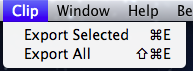
\includegraphics{images/clipMenu.png}
\caption{Exporting Alerts}
\end{figure}

\section{Export Formats}

There are three export formats available, depending on your work- flow.

\subsection{HTML}

The HTML export format will generate an HTML file, with as- sociated
javascript and CSS. This page is designed to be opened in the Safari
browser. In addition to a preview of the clip, you will be presented
with a list of alerts. Clicking each alert will seek to the point within
the video where the alert was triggered.

Keep in mind that the video playback capabilities of the webbrowser does
not allow frame-accurate seeking. When necessary, ScopeBox will err on
the side of seeking just before the alert time, rather than just after.

\subsection{CSV}

The CSV export format will generate a Microsoft Excel compatible CSV
spreadsheet, with an entry for each alert.

\subsection{FCP and FCPX XML}

There are two XML options, for both Final Cut Pro 5 and later, and for
Final Cut Pro X. When opened in Final Cut Pro, this XML will attempt to
load the recorded files associated with each alert. Final Cut Pro will
place markers within the video for each alert. This can be used to
quickly find and correct issues within your source record- ing.

\chapter{ScopeLink}

ScopeLink allows you to monitor the signal from other applications on
your computer, without any special hardware. Once installed, ScopeLink
appears as an output option within supported applica- tions, just like a
traditional hardware output device. ScopeLink requires Mac OS X 10.8
(``Mountain Lion'') or later.

Within ScopeBox, you can add the ScopeLink device from the source menu,
just like any other source.

\begin{figure}[htbp]
\centering
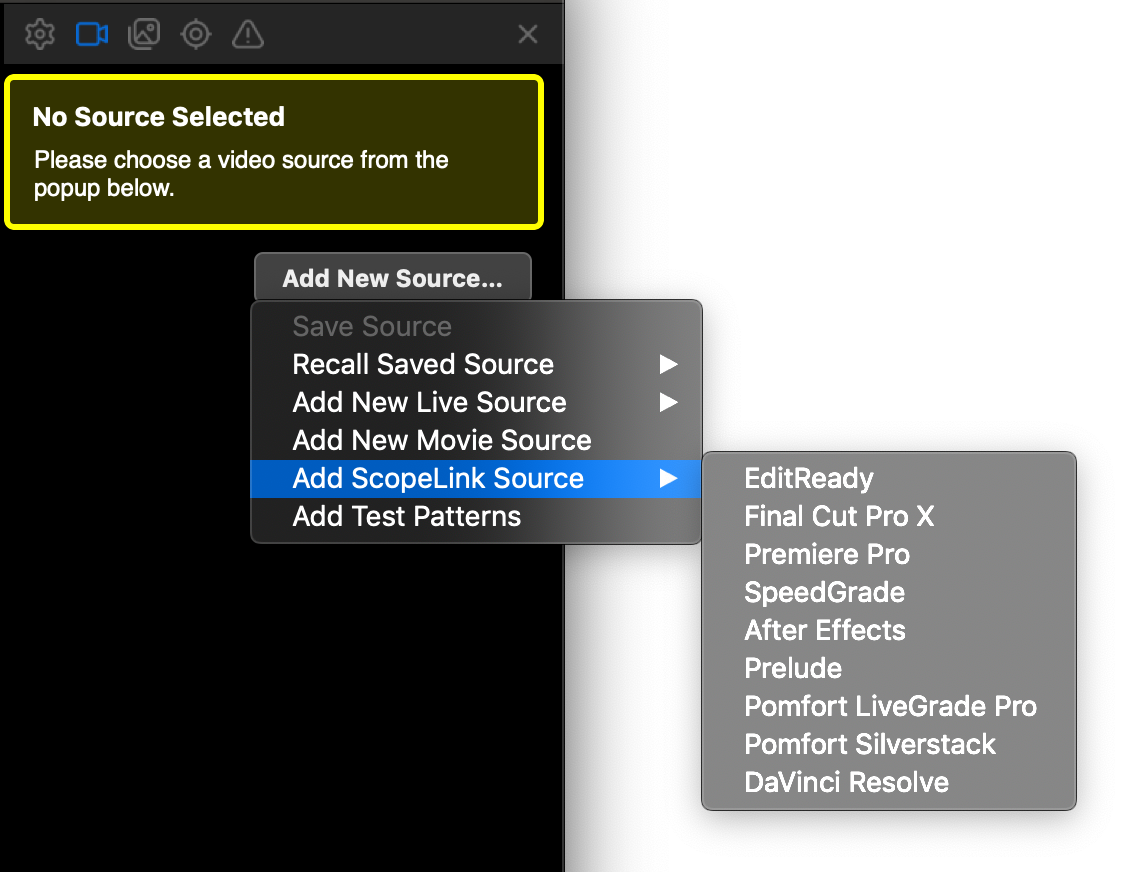
\includegraphics{images/scopelinkSource.png}
\caption{Adding a ScopeLink Source}
\end{figure}

\section{Installing ScopeLink}

Installing ScopeLink requires administrator privileges on your computer.
The first time you attempt to add the ScopeLink source, you'll be
prompted to install ScopeLink. You can manually initiate the
installation by selecting ``Install Additional Software'' from the
ScopeBox menu.

The installation will prompt for your administrator password and install
the ScopeLink software on your system.

\section{Configuring ScopeLink}

After installing, ScopeLink must be activated within the individual
applications you wish to use with ScopeBox. This should only need to be
done once per application.

\subsection{Adobe Premiere and Prelude}

To configure ScopeLink with Adobe Premiere Pro, or Adobe Prelude, begin
by launching the application you wish to configure. Start a new project
(the format doesn't matter). From the menu bar, select ``Adobe
Premiere'' (or ``Adobe Prelude'' and then ``Preferences.'' Within the
preferences dialog, select the ``Playback'' option.

\begin{figure}[htbp]
\centering
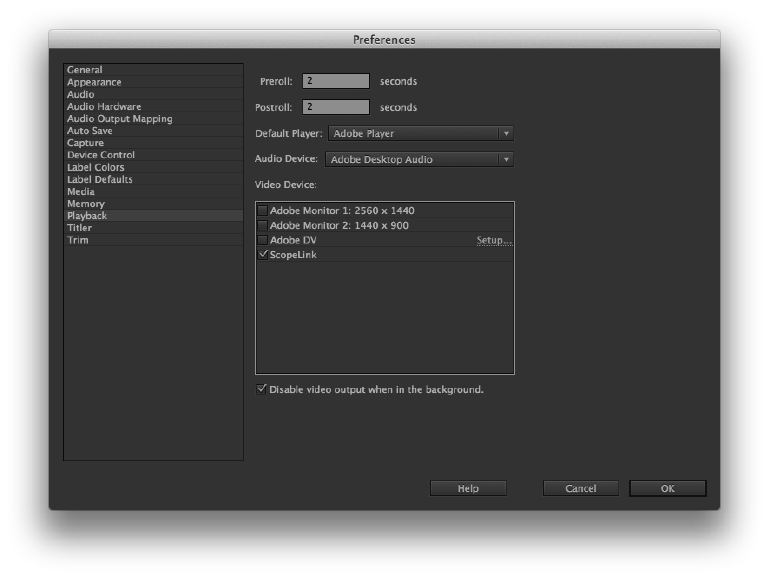
\includegraphics{images/PremierePreferences.png}
\caption{Configuring Adobe Premiere}
\end{figure}

Check the box next to the ScopeLink device. You may also activate other
devices if you wish. Click ``OK,'' and then restart the applica- tion.

When used with Adobe Premiere Pro or Adobe Prelude, ScopeLink will
transmit 8bit Rec. 709 signals, and ScopeBox will default to viewing
within the Rec. 709 colorspace.

\subsection{Adobe After Effects}

To use ScopeLink with Adobe After Effects, begin by launching After
Effects. Select ``Preferences'' from the ``After Effects'' menu, and
then ``View Preview.'' Set ScopeLink as the Output Device and Output
Mode. We recommend checking all of the boxes in the ``output dur- ing''
section.

\begin{figure}[htbp]
\centering
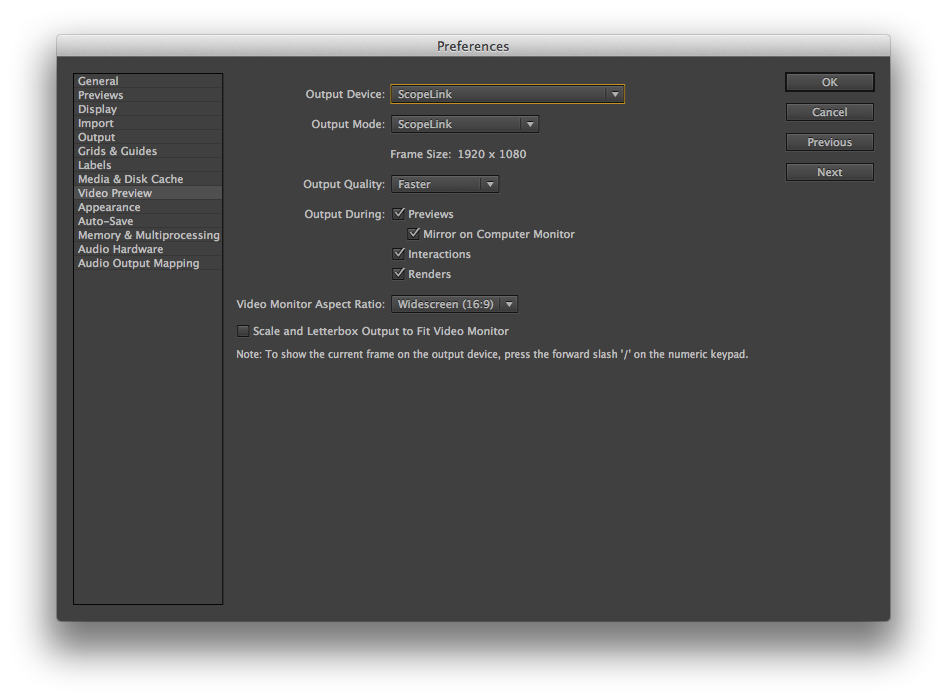
\includegraphics{images/AfterEffects.png}
\caption{Configuring Adobe After Effects}
\end{figure}

Click ``OK'' and then relaunch After Effects.

When used with After Effects, ScopeLink will use the CCIR 601 colorspace
for standard definition frame sizes, and Rec. 709 for high definition
frame sizes.

\subsection{Other Applications}

Other applications which support either QuickTime-based output or Adobe
Transmit-based output may work with ScopeLink. Contact support if you'd
like information on using a specific application with ScopeLink.

\chapter{View Menu}

The View menu allows you to customize the look and feel of the main
ScopeBox window. Each of the major sections of the window - the source
bar, sidebar, and the clip list - can be shown or hidden from the View
menu. In addition, you can save and recall preset palette layouts and
configurations.

\section{Saving a new layout}

To save a custom layout, arrange the palettes as desired and select
``Save Custom Layout\ldots{}''. You will be prompted to name your
layout.

After clicking OK, you will find your newly saved layout in the Layouts
menu.

\section{Restoring a layout}

Choose any of the layouts found in the custom layout section to restore
the main window to this configuration. You can set a default layout,
which will be loaded every time Scope- Box is launched, via the
preferences. If you ever wish to override this default, simply hold the
shift key while launching ScopeBox.

\chapter{Window Menu}

The Window menu provides the Toggle Fullscreen option. Fullscreen mode
hides the dock, menu bar, and all other applications, making ScopeBox
the only visible application.

When in fullscreen mode, the menu bar is revealed when the cursor is at
the top of the screen.

\chapter{Source Diagnostics}

If you're having trouble accessing a particular video device in Scope-
Box, select ``Source Diagnostics'' from the Help menu.

The source diagnostics window will show all of the detected video
devices on your system. If a device has a caution icon next to it, that
means ScopeBox is unable to connect to that device. By selecting the
problem device in the list, you'll see an explanation below of what
reason ScopeBox has for disabling this source.

\begin{figure}[htbp]
\centering
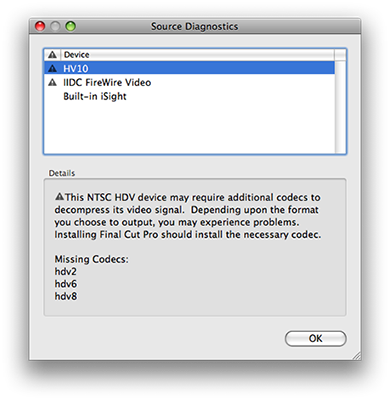
\includegraphics{images/SourceDiagnostics.png}
\caption{An example of Source Diagnostics explaining a source error.}
\end{figure}

There are a few common problems which may cause devices to be disabled,
depending upon their type.

\section{Capture cards and IIDC or USB cameras}

These traditional QuickTime supported devices are disabled most often
due to a conflict with another piece of software on your com- puter.
These devices can only be used by a single application at once.

Applications like FCP must be explicitly told not to open their de-
vice, or launched after ScopeBox has opened the device as a source.
Also, many instant messaging clients will take control of a camera when
launched, even if you're not actively engaged in a video chat.

\section{HDV, or DVCProHD cameras}

In order to take advantage of some FireWire cameras, you must have the
appropriate video codecs installed, which requires installing Final Cut
Pro on the machine. Final Cut Pro installs codecs in ``/Library/
QuickTime'' on your computers hard disk. The Source Diagnostics window
will alert you to which codecs are currently missing that your camera
may require.

Also, many FireWire cameras have modes in which they do not out- put a
signal on the FireWire port. Examples of such cameras include
Panasonic's HVX-200 while in native frame rates (24pN, 30pN) and Sony's
EX-1 while in HQ modes.

\chapter{Performance}

ScopeBox is a high end application and requires a lot of system re-
sources to run properly. The application uses a number of techniques to
actively monitor video processing and allocate CPU resources to ensure
video is captured without frame drops.

If the sources often show the drop frame warning icon, there are a
number of options for increasing available resources and decreasing
resource demand.

\begin{itemize}
\itemsep1pt\parskip0pt\parsep0pt
\item
  Quit other applications
\item
  Verify that there is enough free space on your start up drive (at
  least 1 GB - much more if you are planning to record)
\item
  Lower the preview level of open sources
\item
  Lower the palette count
\item
  Close RGB Histogram and RGB Parade palettes
\item
  Increase sampling on open palettes
\end{itemize}

If none of these actions work then you may need more RAM, a faster video
card or a faster machine.

\chapter{System Requirements}

ScopeBox is a flexible application that can be used with many hard- ware
configurations. System requirements will vary drastically based on your
specific usage and hardware. The following are guidelines for the
minimum system required to run ScopeBox in its default layout.

\begin{itemize}
\itemsep1pt\parskip0pt\parsep0pt
\item
  Intel-base Macintosh
\item
  Graphics card with support for Quartz Extreme.
\item
  1.25 GB of RAM.
\item
  75 MB of disk space.
\item
  External drive for recording.
\item
  Mac OS X 10.6.8 or later.
\end{itemize}

\begin{quote}
\textbf{These minimum requirements are not a guarantee ScopeBox will
work with your exact configuration. Please thoroughly test your hardware
with the trial version before making any decisions. You can download the
trial at }
\end{quote}

\chapter{Troubleshooting}

\section{Using multiple FireWire cameras doesn't work}

Some cameras are unable to coexist properly on the FireWire bus, which
may result in sources not appearing or not behaving as expected. The
cameras sometimes monopolize the FireWire bus, preventing other cameras
from sending video.

As a workaround, you can install a second FireWire bus in your Ma-
cintosh. On laptops this can be done with a PCMCIA or Express- card. On
Mac Pro or PowerMac computers, this can be done via a PCI-e or PCI-x
card.

Please report details about which cameras and computer configura- tions
cause these issues, so we may refine our source documentation. Because
there are hundreds of cameras and nearly infinite combina- tions, we
need help from our users to document this information. Please send your
system configuration via the web form at
\url{http://www.divergentmedia.com/support}

\section{Video is choppy when using multiple cameras}

There are a few things that can cause this problem. First, your computer
may not be powerful enough to decode all of the incoming video streams.
HDV in particular is very CPU intensive. ScopeBox will drop frames on
your palettes in order to optimize recording performance.

Additionally, many FireWire cameras limit your computer's FireWire bus
to 100mbits/second all devices combined. Once you go beyond two or three
cameras, you may have insufficient band- width to add additional
sources. This issue can also be resolved by adding a third party PCI or
express card FireWire bus.

\section{My video input is not showing up / is grayed out/ does not
work}

Make sure your video input isn't in use by another application, check
input cabling, and restart ScopeBox. Verify that your camera is out-
putting video.

Also, verify that you have the proper codecs or drivers installed. While
this is not a absolute assurance the device should work in ScopeBox, you
can confirm your system is set up properly by check- ing to see if the
device works in other QuickTime applications.

Consult Scopebox's Source Diagnostics dialog under the help menu for
additional help determining why ScopeBox may be disabling your device.
See section 18 of this manual for more info of the Source Diagnostics
dialog.

\section{Audio from my DV camera sounds distorted / VU meters only show
one channel of audio}

ScopeBox does not currently support the 12bit audio mode present on some
DV camcorders. If you are experiencing audio distortion from a DV,
DVCam, or DVCProHD camera, switch the device to 16bit mode and the audio
should preview correctly.

\section{I'm using a Panasonic HVX-200 and can't see any video}

When the Panasonic HVX-200 is set to ``pN'' mode, its FireWire port is
disabled. Set the camera to another mode in order for Scope- Box to be
able to utilize it.

There are multiple settings in the HVX which affect the current frame
mode. Be sure to set a non-pN mode under the camera \textgreater{}
recording setup menu. Also, ensure your active scene file has a frame
rate of ``Default'', or this will override the recording setting.

\section{Duplicate frame removal is not working with the HVX-200}

As explained above, there are multiple settings in the HVX which affect
the current frame mode. Be sure you have set a non-pN mode under the
camera \textgreater{} recording setup menu. Also under recording setup,
you need to set ``UB MODE'' to ``FRM.RATE'', which tells the camera to
flag duplicate frames in the video stream, so that Sco- peBox is able to
detect and remove them.

Finally, ensure your active scene file has a frame rate of ``Default'',
or this will override the recording settings above.

\section{All my recordings are out of sync when using Lock to Camera
with my HDV source}

Some cameras may not properly work with ScopeBox's Lock to Camera
feature. Specifically, many HDV cameras reset the timing information in
their video stream at the start of each recording. This reset in the
stream may cause ScopeBox to record audio and video out of sync for the
remainder of that shot. You will need to manually start your ScopeBox
recordings after the HDV camera has had time to begin its record and the
improper timing information has passed.

\chapter{Other Resources}

If you need additional support using ScopeBox, please try the re-
sources listed below.

Support on the Web \url{http://www.divergentmedia.com/scopebox}

Email support
\href{mailto:support@divergentmedia.com}{support@divergentmedia.com}

Phone support toll free - 888.632.0904

\end{document}
